% Options for packages loaded elsewhere
\PassOptionsToPackage{unicode}{hyperref}
\PassOptionsToPackage{hyphens}{url}
%
\documentclass[
]{article}
\usepackage{amsmath,amssymb}
\usepackage{iftex}
\ifPDFTeX
  \usepackage[T1]{fontenc}
  \usepackage[utf8]{inputenc}
  \usepackage{textcomp} % provide euro and other symbols
\else % if luatex or xetex
  \usepackage{unicode-math} % this also loads fontspec
  \defaultfontfeatures{Scale=MatchLowercase}
  \defaultfontfeatures[\rmfamily]{Ligatures=TeX,Scale=1}
\fi
\usepackage{lmodern}
\ifPDFTeX\else
  % xetex/luatex font selection
\fi
% Use upquote if available, for straight quotes in verbatim environments
\IfFileExists{upquote.sty}{\usepackage{upquote}}{}
\IfFileExists{microtype.sty}{% use microtype if available
  \usepackage[]{microtype}
  \UseMicrotypeSet[protrusion]{basicmath} % disable protrusion for tt fonts
}{}
\makeatletter
\@ifundefined{KOMAClassName}{% if non-KOMA class
  \IfFileExists{parskip.sty}{%
    \usepackage{parskip}
  }{% else
    \setlength{\parindent}{0pt}
    \setlength{\parskip}{6pt plus 2pt minus 1pt}}
}{% if KOMA class
  \KOMAoptions{parskip=half}}
\makeatother
\usepackage{xcolor}
\usepackage{graphicx}
\makeatletter
\newsavebox\pandoc@box
\newcommand*\pandocbounded[1]{% scales image to fit in text height/width
  \sbox\pandoc@box{#1}%
  \Gscale@div\@tempa{\textheight}{\dimexpr\ht\pandoc@box+\dp\pandoc@box\relax}%
  \Gscale@div\@tempb{\linewidth}{\wd\pandoc@box}%
  \ifdim\@tempb\p@<\@tempa\p@\let\@tempa\@tempb\fi% select the smaller of both
  \ifdim\@tempa\p@<\p@\scalebox{\@tempa}{\usebox\pandoc@box}%
  \else\usebox{\pandoc@box}%
  \fi%
}
% Set default figure placement to htbp
\def\fps@figure{htbp}
\makeatother
\setlength{\emergencystretch}{3em} % prevent overfull lines
\providecommand{\tightlist}{%
  \setlength{\itemsep}{0pt}\setlength{\parskip}{0pt}}
\setcounter{secnumdepth}{-\maxdimen} % remove section numbering
\usepackage{bookmark}
\IfFileExists{xurl.sty}{\usepackage{xurl}}{} % add URL line breaks if available
\urlstyle{same}
\hypersetup{
  hidelinks,
  pdfcreator={LaTeX via pandoc}}

\author{}
\date{}

\begin{document}

\section{traffic\_air\_quality\_modeling}\label{traffic_air_quality_modeling}

Dynamical systems modeling of transportation systems and their impacts
on urban air pollution. Case of interest: New Delhi, India.

The latest version of the model (as of November 13, 2024) is
\texttt{travel\_4\_1021.ode} in XPPAUT and \texttt{travel\_4.ipynb} in
Julia. It involves two patches connected by two (bidirectional)
corridors.

\subsection{Introduction}\label{introduction}

The transportation system in the National Capital Territory (NCT) of
Delhi, India is a complex network of vehicles, transit lines, and users
of multiple types. Rising air pollution associated with this
transportation system is a major public health challenge, and recent
studies have estimated that poor air quality in Delhi reduces residents'
life expectancy by about 6 years. This system
is bounded by the municipal boundaries of NCT, but the boundaries are
permeable to the movement of air, vehicles, and people across political
boundaries. We conceptualize the transportation system as consisting of
\emph{vehicles} (e.g.~cars, trains, motorcycles, auto-rickshaws,
pedestrians) which travel between \emph{patches} (e.g.~residential
areas, business districts) along \emph{corridors} (e.g.~highways, train
lines) and emit pollutants at a certain rate depending on their travel
speed and congestion levels. To conceptualize the wider
social-ecological context, we can use the Coupled-Infrastructure Systems
(CIS) framework.

\begin{figure}
\centering
\pandocbounded{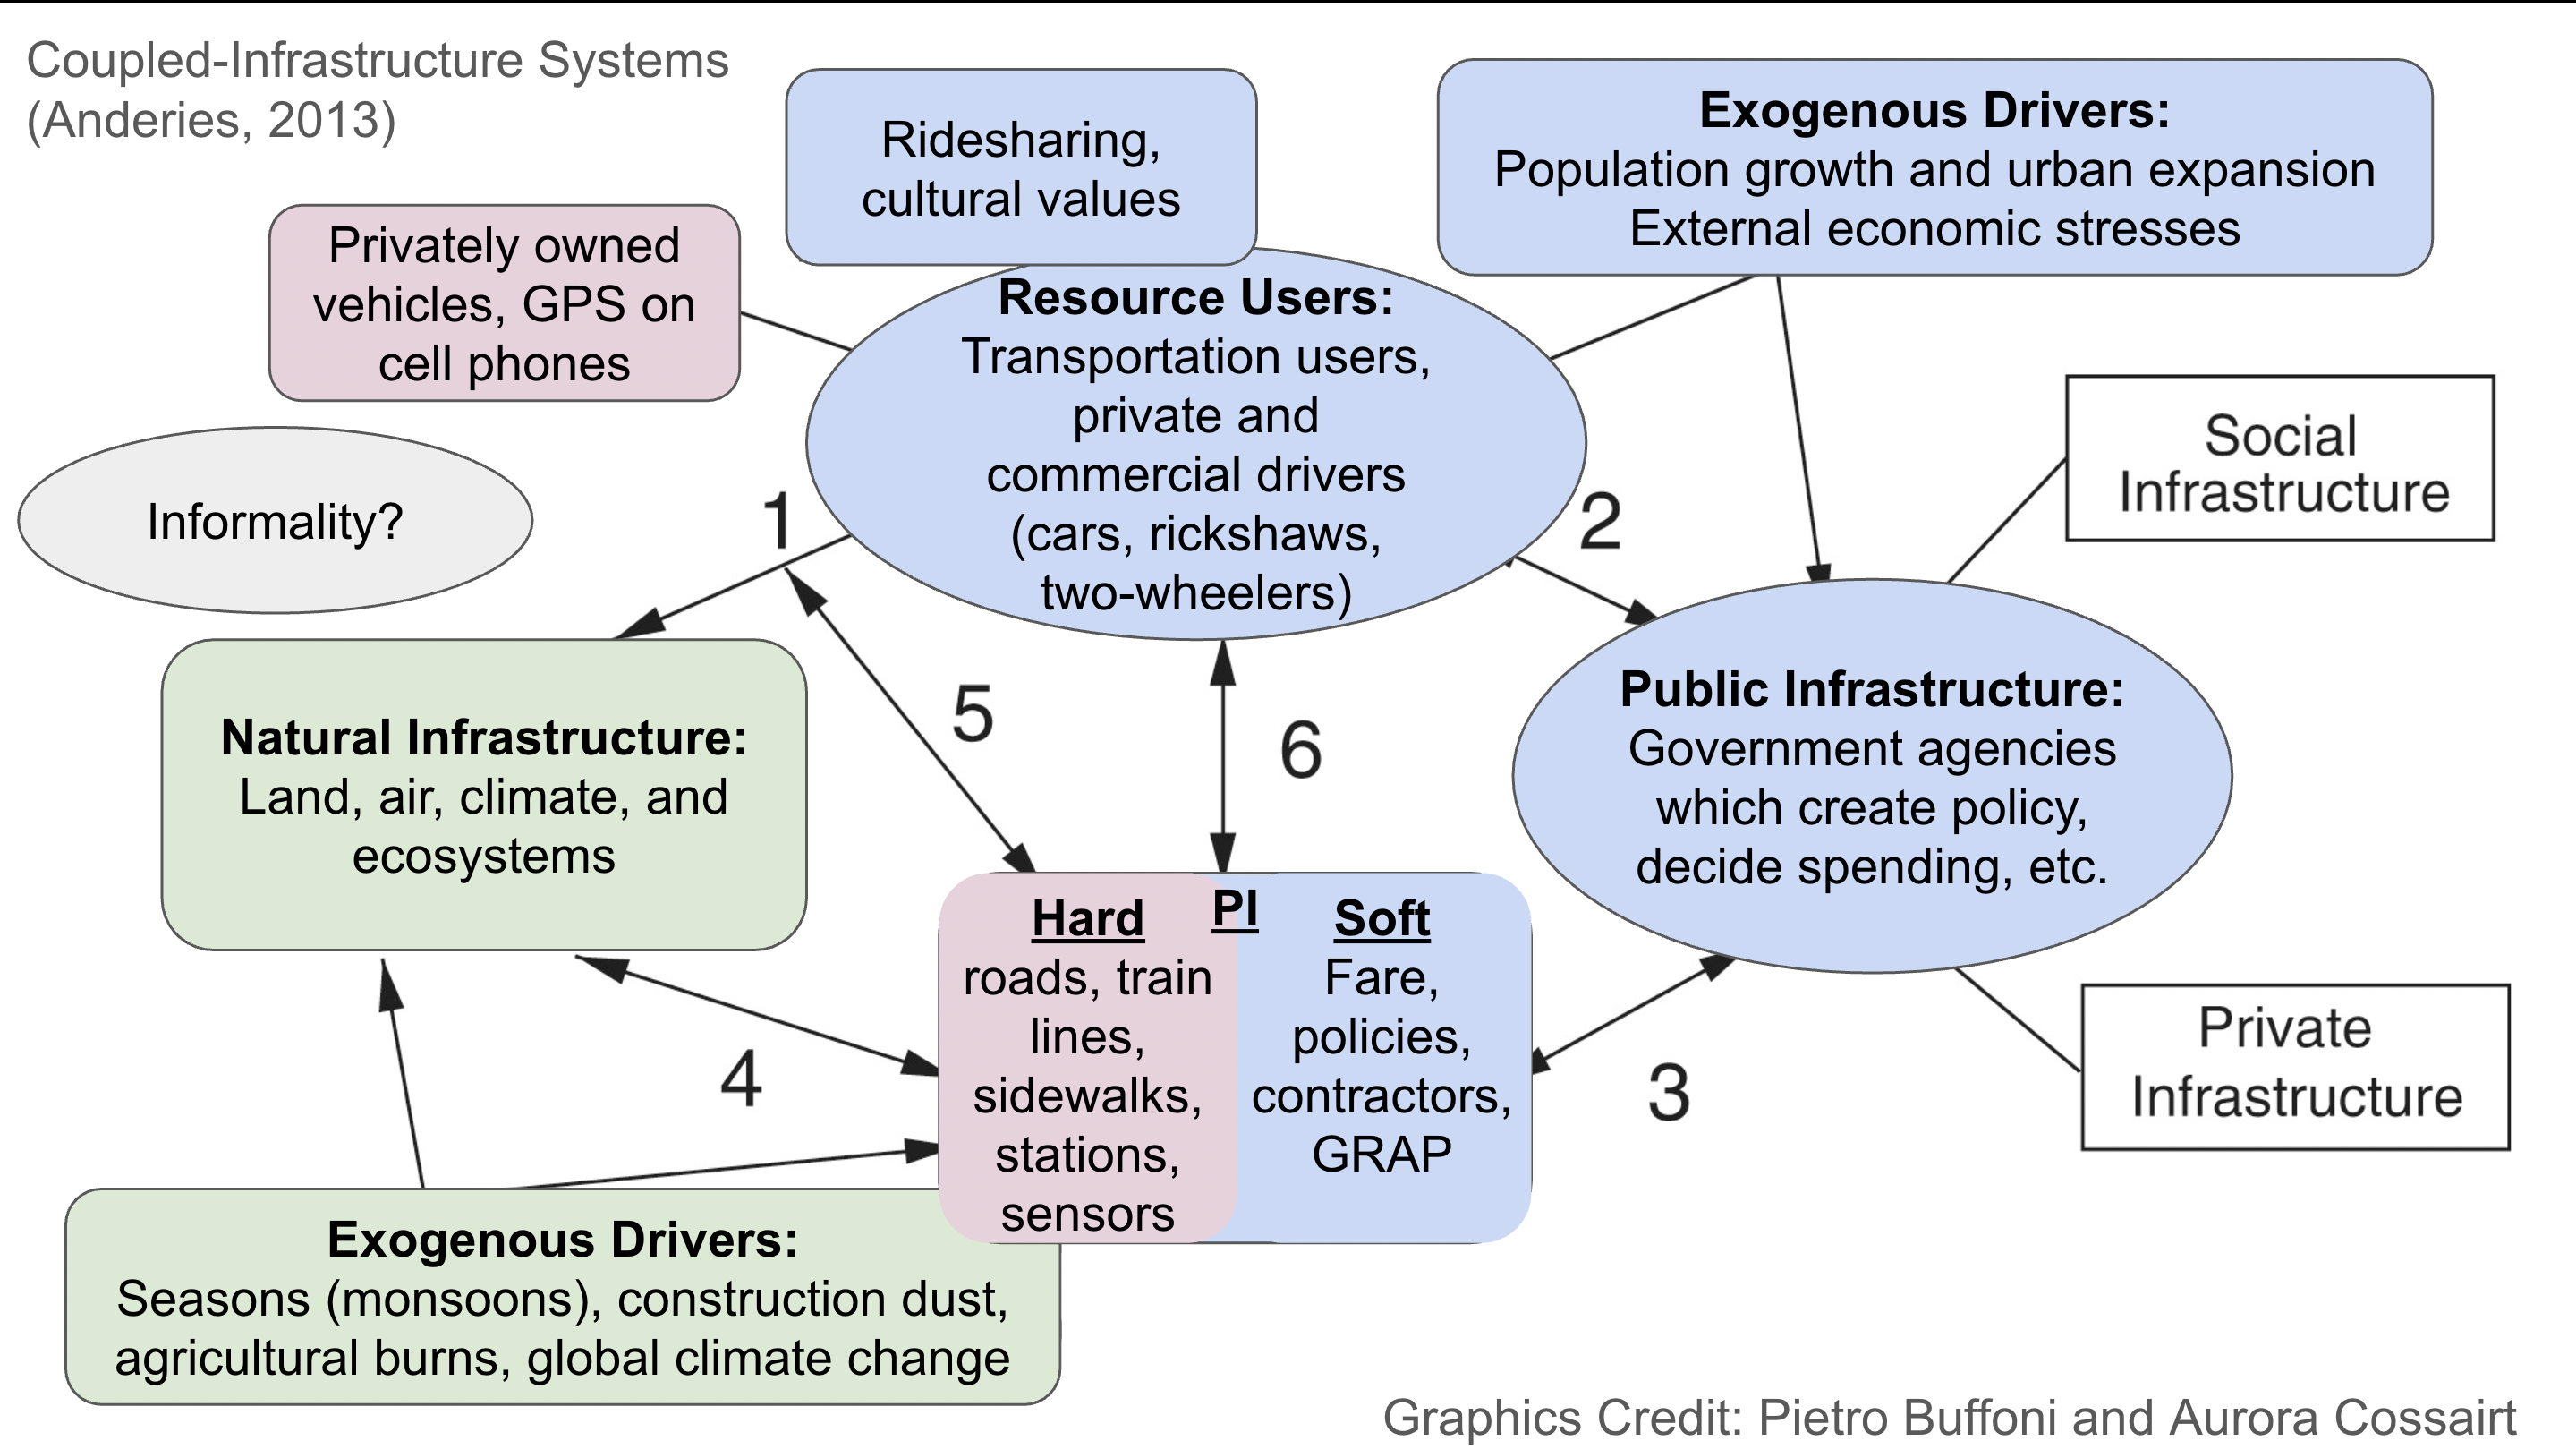
\includegraphics[keepaspectratio]{images/CIS_PIRE_12_2023}}
\caption{alt text}
\end{figure}

\subsection{Research Questions}\label{research-questions}

Our objective is to build a general model of urban mobility systems,
with NCT New Delhi as a prototyping case, to gain insight into the
relationship between mobility infrastructure configurations, governance
policies, and air quality. Specific research questions include: - How
does the overall pollution level compare for a small mobility
infrastructure system (few patches, few corridors) vs a large mobility
infrastructure system (many patches, many corridors)? - What is the
impact on air pollution of increasing capacity of existing roads
(decrease the parameter \(\beta^k\), defined below)? - What is the
impact on air pollution of increasing road connectivity by adding new
corridors while keeping the same number of patches (increase parameter
\(K\), defined below)? - (Future work) How does information flow along
links in the CIS to inform infrastructure investment decisions by PIP?

\subsection{Model Background}\label{model-background}

The concept for this model is shown in \autoref{fig:conceptual_diagram}
for a case with two patches and two connective corridors.
\pandocbounded{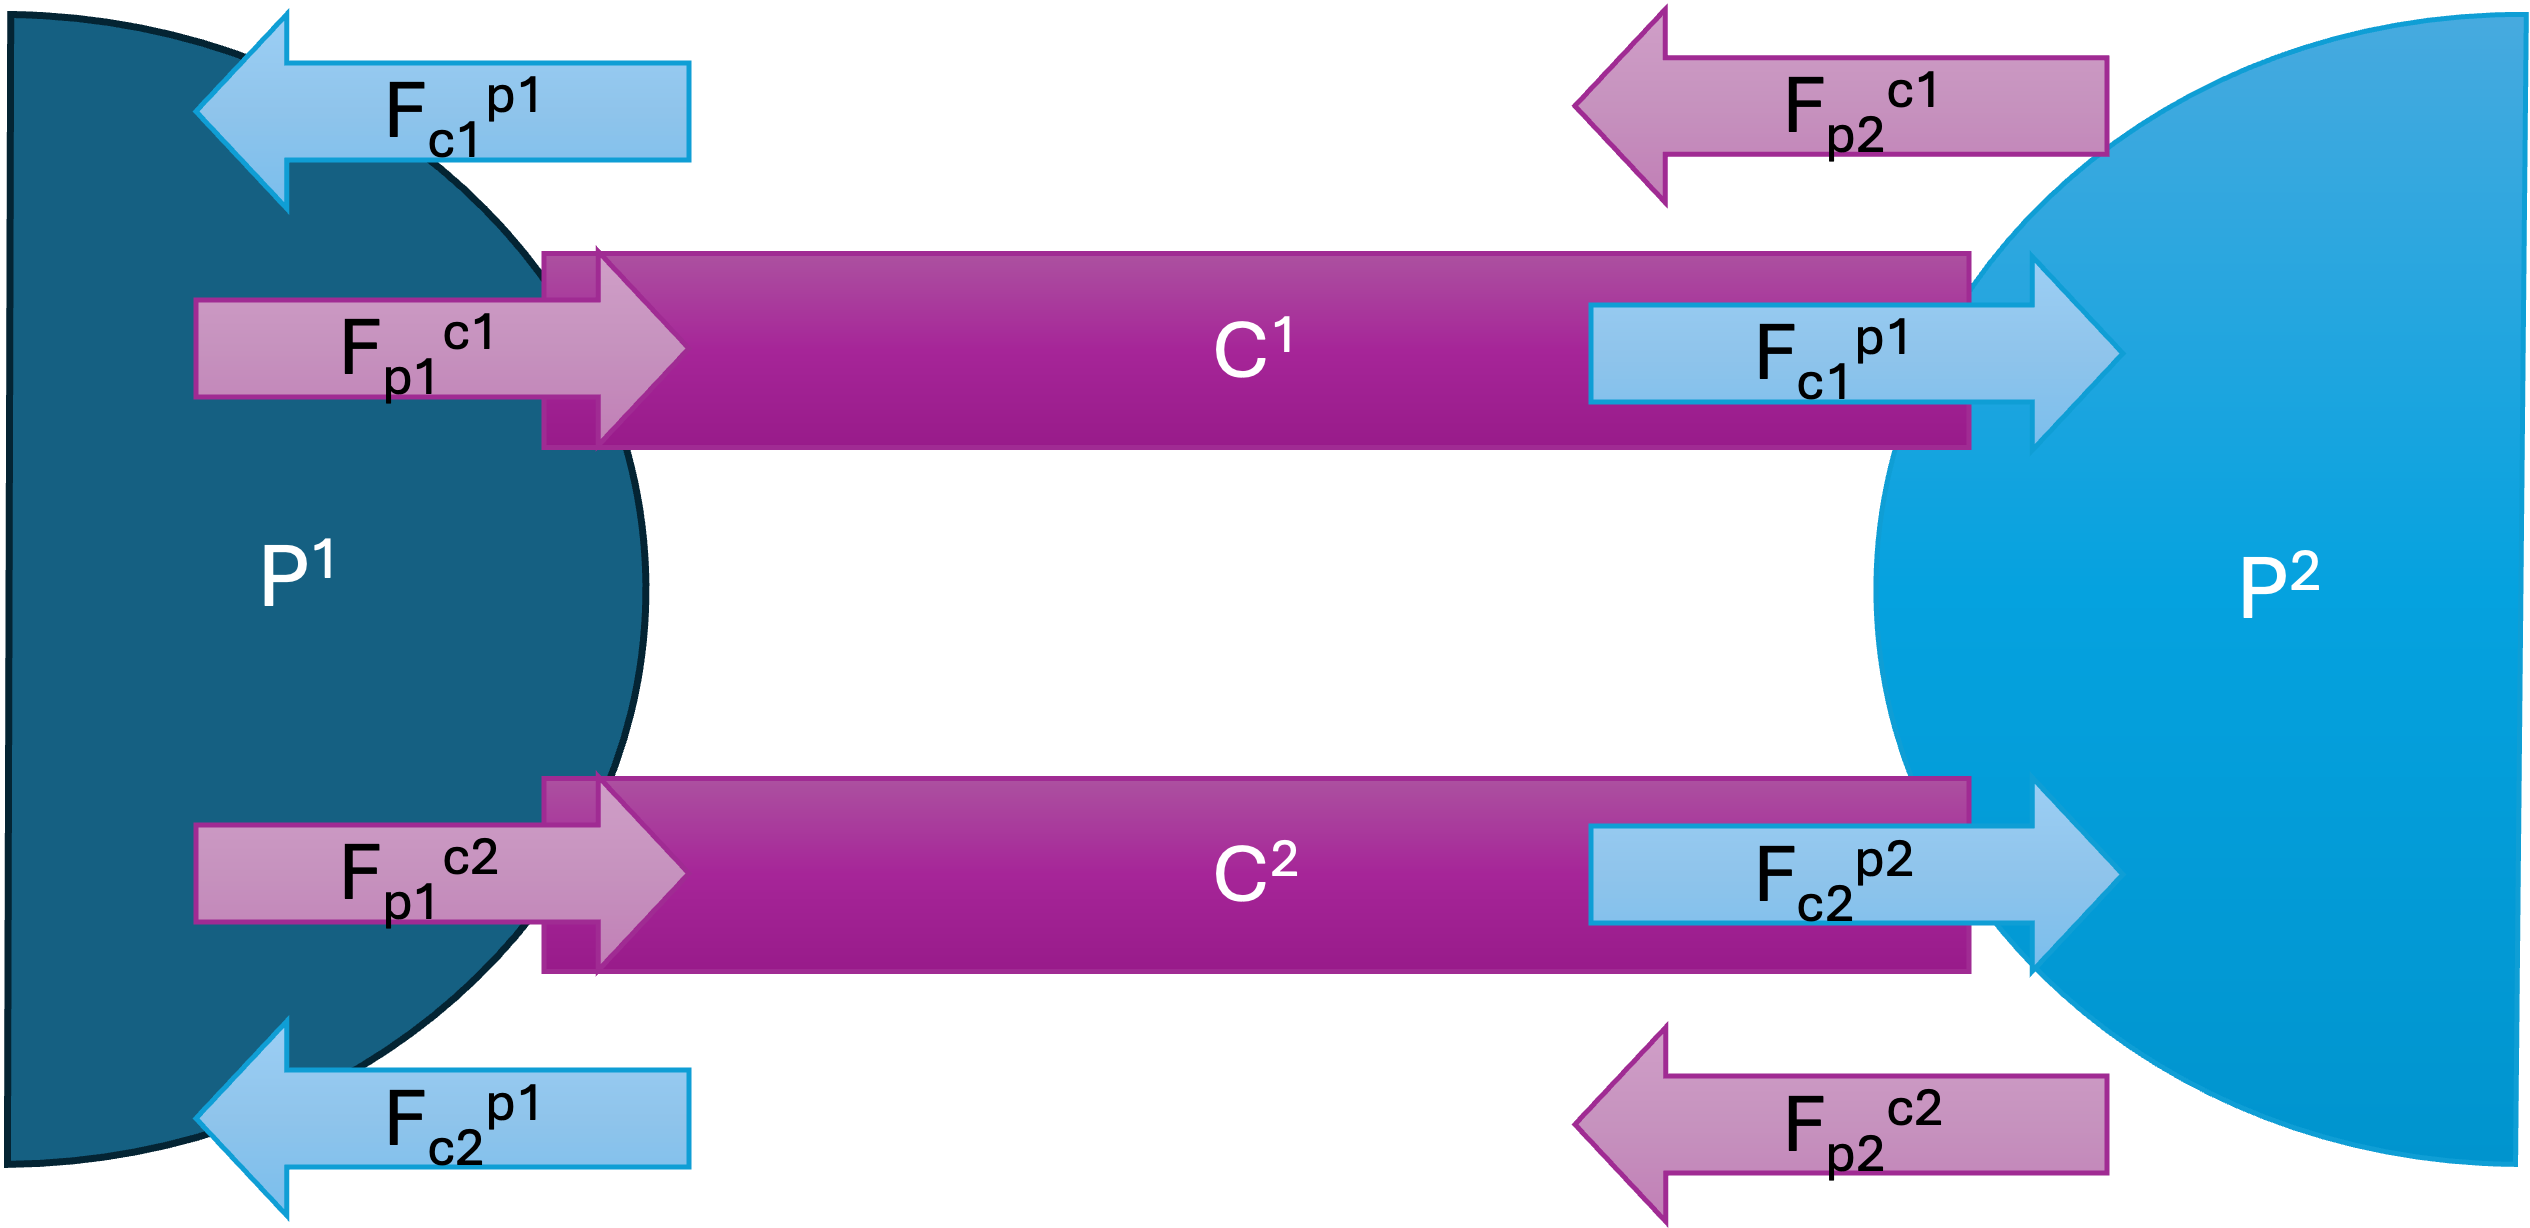
\includegraphics[keepaspectratio]{images/conceptual_framework.png}}

In general, suppose there are \(N\) patches, up to \(K\) corridors
connecting each pair, and 1 total vehicles (this is a normalized value;
we can think of it as a density). The state variables and parameters are
listed below:

\subsubsection{State Variables}\label{state-variables}

\begin{itemize}
\tightlist
\item
  \(P^i\): population in patch \(i\) (units: vehicles)
\item
  \(C^k[i,j]\): population in corridor \(k\), heading from patch \(i\)
  to patch \(j\) (units: vehicles)
\end{itemize}

These state variables are countable populations which could in theory be
measured at a point in time.

\subsubsection{Parameters}\label{parameters}

\begin{itemize}
\tightlist
\item
  \(\beta^k[i,j]\): Road congestion factor (inverse road capacity) for
  corridor \(k\). Analogous to ``resistance'\,' in an electrical wire.
  Think of congestion as the ratio of vehicles on the road to the jam
  capacity of that road: \(C^k[i,j] / C^k_{jam}[i,j]\). Therefore,
  \(\beta^k[i,j] = 1 / C^k_{jam}[i,j]\), and \(\beta^k[i,j]=0\) would
  imply infinite road capacity. (units: 1/vehicles)
\item
  \(\alpha^i\): aversion to congestion for travelers from patch \(i\).
  Given \(\beta_k C^k_{i,j}\),
  \(\uparrow \alpha \Rightarrow \downarrow\) new travelers. (unitless)
\item
  \(O^P[i]\): Percentage of population in patch \(i\) who want to
  travel. (unitless) \textbackslash end\{itemize\}
\end{itemize}

These parameters describe infrastructure capacity (such as the width of
a highway) and social behavior of travelers. These quantities are likely
to change on a time scale of months to years, whereas our model is
focused on traffic flows on a time scale of minutes and hours, so we can
treat the above quantities as parameters.

\subsubsection{Conservation law}\label{conservation-law}

Here the total number of vehicles is conserved.

\subsubsection{Relationships between
variables}\label{relationships-between-variables}

Because of the conservation law, the change in number of vehicles in any
node (a patch, corridor, urban sponge, etc.) is determined by
\emph{flow-in} minus \emph{flow-out}. The speed of fluxes into and out
of corridors is density dependent.

\begin{itemize}
\tightlist
\item
  \(F^{\rightarrow k}[i,j]\): flux from patch \(i\) into corridor \(k\),
  with an ultimate destination of patch \(j\).
\item
  \(F^{k\rightarrow}[i,j]\): flux from corridor \(k\) into patch \(j\),
  where the origin was \(i\).
\end{itemize}

\subsection{Formal Model}\label{formal-model}

For a general system of \(N\) patches, and up to \(K\) connecting
corridors for each pair of patches, we will use the following notation:

The number of vehicles in each patch \(P^i\) is given by \(P[i]\).


\begin{align}
  P &= 
  \begin{pmatrix}
      1 \\
      2 \\
      ... \\
      n
  \end{pmatrix}
\end{align}


Number of vehicles in a corridor \(C^k\) heading from patch \(i\) to
patch \(j\) is given by \(C^k[i,j]\). For example, suppose maximum of
one connecting corridor for each pair of patches, and assume no
self-connected patches, the matrix \(C^k\) is:

\begin{align*}
    C^k &=
    \begin{pmatrix}
        0 & 1 \rightarrow 2 & 1 \rightarrow 3 & ... & 1 \rightarrow n \\
        2 \rightarrow 1 & 0 & 2 \rightarrow 3 & ... & 2 \rightarrow n \\
        ... & ... & ... & ... & ... \\
        n \rightarrow 1 & n \rightarrow 2 & n \rightarrow 3 & ... & 0
    \end{pmatrix}
\end{align*}

If \(K>1\), we may have multiple matrices \(C^k[i,j]\) (one for each
\(k\)), or the \(C\) matrix may be three dimensional with indices
\([i,j,k]\).

For fluxes from patches into corridors, we also need a matrix with three
dimensions \(i,j,\) and \(k\). \(F^{\rightarrow k}[i,j]\) means flux
from patch \(i\) into corridor \(k\), with an ultimate destination of
patch \(j\).


\begin{align*}
    F^{\rightarrow k}[i,j] &=
    \begin{pmatrix}
        0 & p1 \rightarrow ck (\rightarrow p2) & p1 \rightarrow ck (\rightarrow p3) & ... & p1 \rightarrow ck (\rightarrow pn) \\
        p2 \rightarrow ck (\rightarrow p1) & 0 & p2 \rightarrow ck (\rightarrow p3) & ... & p2 \rightarrow ck (\rightarrow pn) \\
        ... & ... & ... & ... & ... \\
        pn \rightarrow ck (\rightarrow p1) & pn \rightarrow ck (\rightarrow p2) & pn \rightarrow ck (\rightarrow p3) & ... & 0
    \end{pmatrix}
\end{align*}


Meanwhile, \(F^{k\rightarrow}[i,j]\) means fluxes from corridor \(k\)
into patch \(j\), where the origin was \(i\).


\begin{align*}
    F^{k \rightarrow}[i,j] &=
    \begin{pmatrix}
        0 & (p1 \rightarrow) ck \rightarrow p2 & (p1 \rightarrow) ck \rightarrow p3 & ... & (p1 \rightarrow) ck \rightarrow pn \\
        (p2 \rightarrow) ck \rightarrow p1 & 0 & (p2 \rightarrow) ck \rightarrow p3 & ... & (p2 \rightarrow) ck \rightarrow pn \\
        ... & ... & ... & ... & ... \\
        (pn \rightarrow) ck \rightarrow p1 & (pn \rightarrow) ck \rightarrow p2 & (pn \rightarrow) ck \rightarrow p3 & ... & 0
    \end{pmatrix}
\end{align*}


\subsubsection{Governing differential
equations}\label{governing-differential-equations}

The system of differential equations governing this system can be
written:


\begin{align}
    \frac{dP^i}{dt} &= \sum_{k=1}^K \sum_{j=1}^N F^{k\rightarrow}[j,i] - \sum_{k=1}^K \sum_{j=1}^N F^{\rightarrow k}[i,j] \\
    \frac{dC^{k}\_{ij}}{dt} &= \sum_{k=1}^K F^{\rightarrow k}[i,j] - \sum_{k=1}^K F^{k\rightarrow}[i,j]
\end{align}


with the conservation law:


\begin{align}
    1 &= \sum_{i=1}^N P[i] + \sum_{k=1}^K \sum_{i=1}^N \sum_{j=1}^N C^k[i,j]
\end{align}


The equations for fluxes into and out of corridors are as follows.

\subsubsection{Fluxes from patches to
corridors}\label{fluxes-from-patches-to-corridors}


\begin{align}
    F^{\rightarrow k}[i,j] &= \exp{(-\alpha[i] * \beta^k[i,j] * C^k[i,j])} * O^{P}[i] * P[i]
\end{align}


This equation states that the number of vehicles which flow from patch
\(i\) into corridor \(k\) with a final destination of patch \(j\)
depends positively on the current number of vehicles in patch \(i\) who
want to leave (\(O^{P}[i] * P[i]\)), and inversely on the current
congestion level (\(\beta^k[i,j] C^k[i,j]\)), with the strength of
aversion to congestion controlled by the factor \(\alpha[i]\).

\subsubsection{Fluxes from corridors to
patches}\label{fluxes-from-corridors-to-patches}


\begin{align}
    F^{k \rightarrow}[i,j] &= \exp{(-\beta^k[i,j] * C^k[i,j]}) * C^k[i,j]
\end{align}


This equation says that number of vehicles flowing out of corridor \(k\)
into patch \(j\), with an origin of patch \(i\), is proportional to the
number of cars on the road \(C^k[i,j]\) and inversely related to the
congestion on the road \(\beta^k[i,j] * C^k[i,j]\). There is no factor
controlling sensitivity to congestion, because we assume anyone already
traveling in a corridor will exit (reaching their final destination) at
the earliest opportunity.

\subsubsection{Predicting emissions from traffic
density}\label{predicting-emissions-from-traffic-density}

Given a traffic density \(C^k[i,j]\) on a given corridor which has jam
density \(C^k_{jam}[i,j] = 1 / \beta^k[i,j]\), we can compute average
speeds from an alternative version of \textbf{Greenshield's model} and
then predict emissions / vehicle using the \textbf{U-shaped curve}.

\paragraph{Traffic density to average
speed}\label{traffic-density-to-average-speed}

First, to compute average vehicle speeds, we will use an alternative to
Greenshield's law. The typical Greenshield's model states:


\begin{equation}
    v^k[i,j] = v^k_{free}[i,j] - \left(\frac{v^k_{free}[i,j]}{C^k_{jam}[i,j]}\right) C^k[i,j]
\end{equation}


where \(v^k_{free}[i,j]\) is the free-flow speed and \(C^k_{jam}[i,j]\)
is the jam density in corridor \(k\) connecting patches \(i\) and \(j\).
This formula codifies a linear relationship between velocity and
density, where average speeds go to zero exactly at
\(C^k[i,j] = C^k_{jam}[i,j]\), and the average speed is the free flow
velocity \(v^k[i,j]\) only in the edge case where \(C^k[i,j] = 0\).

A more realistic version of this model would show nearly free flow
speeds for a range of traffic density, followed by a sharp drop in
average speeds at a certain congestion threshold \(C^k_{thresh}[i,j]\),
and then average speeds asymptotically approaching zero. We can
represent such a relationship with the following function:


\begin{align*}
    v^k[i,j] &= - \frac{v^k_{free}[i,j]}{\pi} \arctan{a(C^k[i,j] - C^k_{thresh}[i,j])} + \frac{v^k_{free}[i,j]}{2} 
\end{align*}


where \(a\) is a parameter that controls the speed at which congestion
decreases average speeds, \(C^k_{thresh}[i,j]\) is the vehicle density
value for which average speeds are \(\frac{1}{2} v^k{free}[i,j]\). If we
say \(C^k_{thresh}[i,j] = \frac{1}{2}C^k_{jam}[i,j]\), then an
equivalent formula is:


\begin{align}
    v^k[i,j] &= - \frac{v^k_{free}[i,j]}{\pi} \arctan{a(C^k[i,j] - \frac{C^k_{jam}[i,j]}{2})} + \frac{v^k_{free}[i,j]}{2}
\end{align}


Therefore, the road congestion parameter can now be written
\(\beta^k[i,j] = \frac{1}{2 C^k_{thresh}[i,j]}\). The shape of the
function \autoref{eq:alternative_greenshields} is illustrated in
\autoref{fig:greenshield} in purple, compared to the original
Greenshield's model \autoref{eq:greenshield} in green.

\begin{figure}
\centering
\pandocbounded{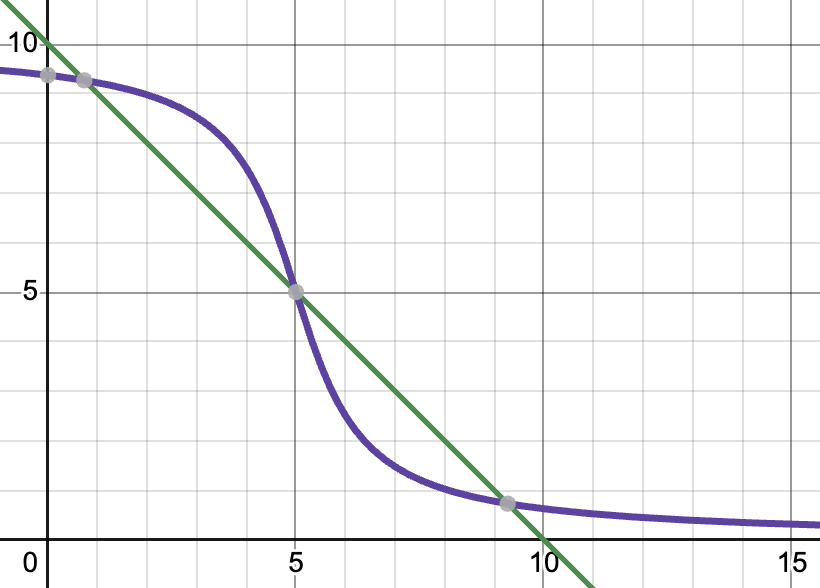
\includegraphics[keepaspectratio]{images/alternative_greenshields_model_2}}
\caption{alt text}
\end{figure}

\paragraph{Average speeds to emission
rates}\label{average-speeds-to-emission-rates}

With average vehicle speeds in hand, we can estimate emission rates
using the U-shaped curve. This empirical function depends on particular
vehicle types, engine and fuel types, and location, and it relates CO2
emission rates (grams / unit distance) with average vehicle speeds (unit
distance / time). We assume that very low average speeds (e.g.~5mph) are
associated with stop-and-go traffic, and therefore high emission rates.
Meanwhile, very high average speeds (e.g.~\(> 85\) mph) also lead to
high emissions because of the energy required to sustain high speeds,
and how quickly a vehicle can travel many miles. An example is shown in
\autoref{fig:u-shaped_curve} with data from California. We will eventually procure similar data for
NCT Delhi -- for now, we can use the California data as a proxy.

Given an array for the U-shaped curve \(E\_per\_v\), total emission
rates \(g / hr\) at any given time for a mass of vehicles will be
emissions per vehicle (g / vehicle) times average vehicle speeds
(distance / time) times density of vehicles (vehicles):


\begin{align*}
    Emissions = E\_{{per}\_v}[v^k[i,j]] * v^k[i,j] * C^k[i,j]
\end{align*}


\subsection{Formal model for demo case: two patches, two
corridors}\label{formal-model-for-demo-case-two-patches-two-corridors}

For the simple system with two patches and two corridors shown in
\autoref{fig:conceptual_diagram}, the system of equations is as follows:


\begin{align*}
    \frac{dP^1}{dt} &= F_{c1}^{p1} + F_{c2}^{p1} - F_{p1}^{c1} - F_{p1}^{c2} \\
    \frac{dP^2}{dt} &= F_{c1}^{p2} + F_{c2}^{p2} - F_{p2}^{c1} - F_{p2}^{c2} \\
    \frac{dC^{1}\_{12}}{dt} &= F_{p1}^{c1} - F_{c1}^{p2} \\
    \frac{dC^{1}\_{21}}{dt} &= F_{p2}^{c1} - F_{c1}^{p1} \\
    \frac{dC^{2}\_{12}}{dt} &= F_{p1}^{c2} - F_{c2}^{p2} \\
    \frac{dC^{2}\_{21}}{dt} &= F_{p2}^{c2} - F_{c2}^{p1}
\end{align*}


Conservation law:


\begin{align*}
    1 &= P^1 + P^2 + C^1_{12} + C^1_{21} + C^2_{12} + C^2_{21}
\end{align*}


Fluxes from patches to corridors depend on 1) population of patch \(i\)
interested in becoming travelers (\(O^{Pi} * P^i\)), 2) current levels
of congestion (\(\beta_1 * C^1_{12}\)), and 3) how averse to congestion
are the potential travelers (\(\alpha_i\)).


\begin{align*}
    F_{p1}^{c1} &= \exp{(-\alpha_1 * \beta_1 * C^1_{12})} * O^{P1} * P^1 \\
    F_{p1}^{c2} &= \exp{(-\alpha_1 * \beta_2 * C^2_{12})} * O^{P1} * P^1 \\
    F_{p2}^{c1} &= \exp{(-\alpha_2 * \beta_2 * C^1_{21})} * O^{P2} * P^2 \\
    F_{p2}^{c2} &= \exp{(-\alpha_2 * \beta_2 * C^2_{21})} * O^{P2} * P^2 \\
\end{align*}


Fluxes from corridors to patches depends on the current population in a
patch


\begin{align*}
    F_{c1}^{1} &= \exp{(-\beta_1 * C^1_{21})} * C^1_{21} \\
    F_{c1}^{2} &= \exp{(-\beta_1 * C^1_{12})} * C^1_{12} \\
    F_{c2}^{1} &= \exp{(-\beta_1 * C^2_{21})} * C^2_{21} \\
    F_{c2}^{2} &= \exp{(-\beta_1 * C^2_{12})} * C^2_{12} \\
\end{align*}


Average speeds are then calculated as follows:

\begin{verbatim}
  using Interpolations

  # Calculate speeds from densities
  v_f = 90 # free-flow velocity, 90 km/hr
  k_jam_C1 = 1 / \beta_1
  k_jam_C2 = 1 / \beta_2
  k_half_C1 = k_jam_C1 / 2
  k_half_C2 = k_jam_C2 / 2

  # Function to calculate average speeds using alternative Greenshield's model
  function calc_space_mean_speed_alternative(v_f, k, k_half; a=1)
    u_s = - (v_f / pi) * atan(a*(k - k_half)) + (v_f / 2)
    return u_s > 0 ? u_s : 0
  end

  # Calculate average vehicle speeds for C1 and C2
  C1_speeds = calc_space_mean_speed_alternative.(v_f, pop_C1, k_half_C1)
  C2_speeds = calc_space_mean_speed_alternative.(v_f, pop_C2, k_half_C2)
\end{verbatim}

And finally, emission rates are calculated:

\begin{verbatim}
    # Make a U-shaped curve
    start = 5 # speeds in mph, from California paper
    my_step = 5
    stop = 100
    mph_to_kmh = 1.60934
    speed_arr = collect(start:my_step:stop) * mph_to_kmh # convert mph to kmh
    emissions_arr = [1200, 950, 700, 500, 425, 350, 325, 310, 309, 308, 308, 308, 309, 320, 330, 350, 375, 400, 450, 550] * mph_to_kmh
    plot(speed_arr, emissions_arr)
    
    # Define an interpolation function to get emission rate (g / distance) for particular average speeds
    interp_fn = linear_interpolation(speed_arr, emissions_arr, extrapolation_bc=Line())

    # Function to calculate emission rate (g / hour) for given average speeds
    function calc_emissions_from_speed(vehicle_pop_arr, my_speed_arr, interp_fn)
        interpolated_emission_per_vehicle = interp_fn(my_speed_arr)
        emissions = interpolated_emission_per_vehicle .* my_speed_arr .* vehicle_pop_arr
        return emissions
    end

    # Calculate emissions for C1 and C2
    C1_emissions = calc_emissions_from_speed(pop_C1, C1_speeds, interp_fn)
    C2_emissions = calc_emissions_from_speed(pop_C2, C2_speeds, interp_fn)
\end{verbatim}

\subsection{Analysis}\label{analysis}

For the demo case, we find traffic flows and resulting emissions for 100
times steps with parameters \(O^p[1]=1, O^p[2]=0\),
\(\alpha_1 = \alpha_2 = 1\), and \(\beta^1[1,2] = 10\),
\(\beta^2[1,2] = 60\). That is, everyone wants to leave patch 1, no one
wants to leave patch 2, all travelers have equal tolerance for
congestion, and corridor 1 has much higher capacity than corridor 2. We
start with all vehicles in patch 1 and no travelers in any of the other
patches or corridors. The traffic flows for this case are shown in
\autoref{fig:traffic_flows_1}. We see more travelers choosing corridor 1
over corridor 2, and the rush hour (period of high traffic) in corridor
1 is about 45 time steps, compared to corridor 2's rush hour of more
than 100 time steps.

\begin{figure}
\centering
\pandocbounded{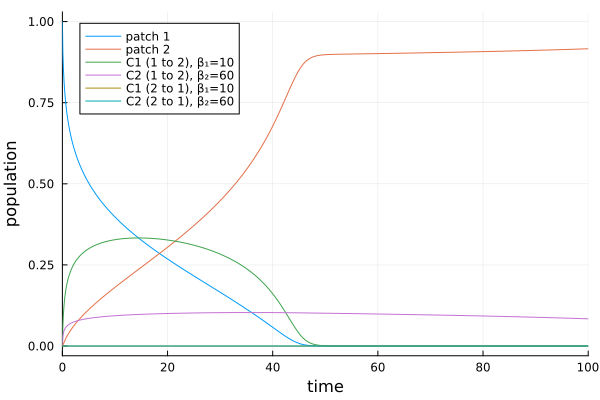
\includegraphics[keepaspectratio]{julia_model/traffic_flows_1}}
\caption{alt text}
\end{figure}

The associated emissions over time for each corridor is shown in
\autoref{fig:emissions}. We notice the curve for emissions rates for
each corridor is almost identical to its associated population curve,
with a bit of discretization. The final step (not shown) to calculate
total emissions for a given part of the day is the integrate the area
under the emissions curve for time \(a\) to time \(b\).

\begin{figure}
\centering
\pandocbounded{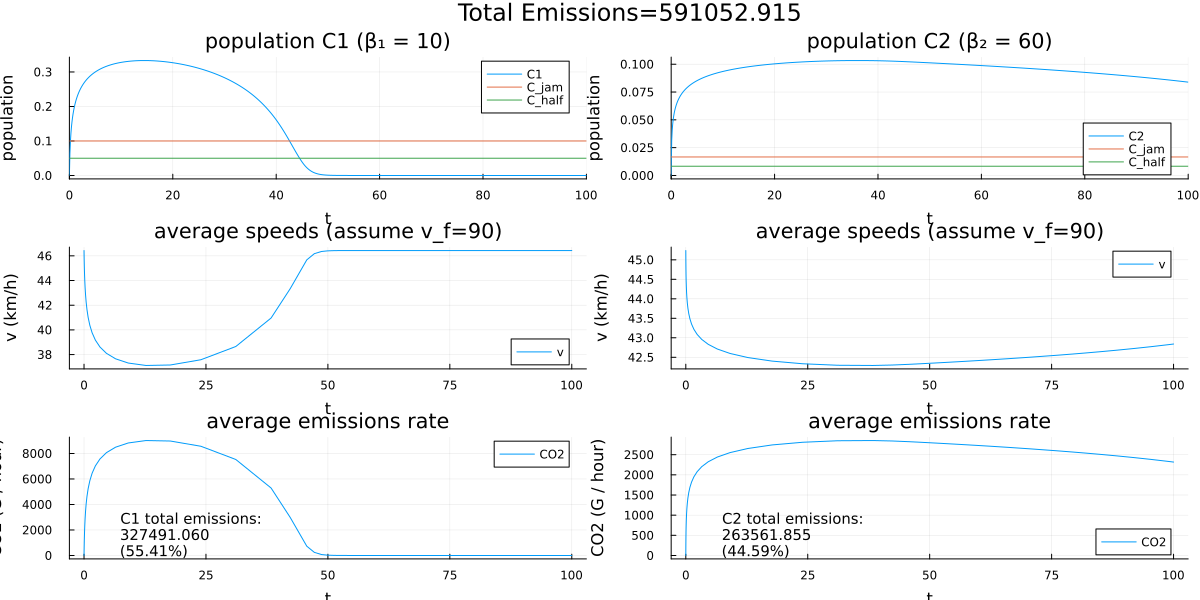
\includegraphics[keepaspectratio]{julia_model/julia_plots/congestion_to_emissions_C1_and_C2_β₁_10_β₂_60}}
\caption{alt text}
\end{figure}

\subsection{Discussion/Conclusion}\label{discussionconclusion}

This exercise showed me the importance of dimensional analysis to
developing a realistic model. At multiple phases of this project, I
found myself questioning the realism of the model, or struggling to
connect my first principles model with other models (such as
Greenshield's model). The solution always came from a careful assessment
of how to interpret each variable and parameter in terms of its units.

At the moment, I am not satisfied with this model for several reasons: -
The assumption that emissions depend on average speeds according to a
simple U-shaped function rests on the logic that lower average speeds
indicate stop-and-go traffic conditions. This is unsatisfying because
emissions really depend on how often drivers hit the accelerator. Two
trips might have the same average speed but very different emission
rates depending on driving patterns. - Additionally, the current
analysis pipeline of vehicle population \(\rightarrow\) average speeds
\(\rightarrow\) emissions implies a linear relationship between
population density and emission rates at each time. This seems overly
simplistic, and it doesn't suggest any interesting properties about how
travel infrastructure relates to emissions.

Future versions of the model should also consider more sophisticated
social-ecological interactions. For instance: - Increasing road capacity
(e.g.~by widening highways) can induce additional demand (higher
\(O^P\)). Our model currently does not consider non-static demand. -
Corridors that represent highways, smaller streets, and railways should
likely be governed by different dynamical equations (e.g.~trains depart
in discrete increments, there is no continuous flow in and out). - We
should model heterogeneous traffic flows, such as highways used by cars,
trucks, motorcycles, auto-rickshaws, cyclists, and pedestrians who may
be using the same corridor simultaneously.

Eventually, we hope to flesh out the links in the CIS model that connect
this formal model of hard urban infrastructure to policy decisions. It
would be particularly useful to identify how information about road
conditions and emissions flow between nodes and influence the
infrastructure investment decisions of PIPs.

\end{document}
